\section{$\beta$-glucuronidase Experiment}
\subsection{Experimental Procedures}
\begin{enumerate}
	\item Prepare phosphate buffer\footnote{Calculated by AAT Bioquest} (0.1 M, pH=6.8, 50 mL): 
	\begin{itemize}
		\item Prepare 40 mL of distilled water in a volumetric bottle.
		\item Add 0.656 g of monosodium phosphate to the solution.
		\item Add 0.352 g of disodium phosphate to the solution.
		\item Adjust pH using HCl or NaOH.
		\item Add distilled water until volume is 0.05 L.
	\end{itemize}
	
	\item Prepare enzyme solution (4 mg/mL): dissolve 0.0060 g $\beta$-Glucuronidase in 1.5 mL phosphate buffer. Store in -20\degree C freezer\footnote{Sigma Product Information: A solution in 75 mM phosphate buffer, pH 6.8, \textgreater 5 mg/ml may be stored at -20 \degree C for up to 2 months with little or no loss of activity.}
	\item Prepare urine samples: thaw samples in the fridge and centrifuge (3000 rpm, 2 min). Prepare 2 Eppendor tubes, one labeled as 'blank', one as 'treatment'. Transfer 100 \si{\micro\litre} to each Eppendorf tube.
	\item Enzymatic hydrolysis reaction: add 50 \si{\micro\liter} phosphate solution to 'blank', 50 \si{\micro\liter} enzyme solution to eppendorf tube, incubate in 37 \degree C for 1.5 h.
	\item Denature enzymes to terminate the reaction
	\begin{itemize}
		\item Add 50 \si{\micro\liter} MeOH to the solution and vortex mix for 1 min
		\item Centrifuge at 3000 rmp for 3 min
		\item Add solvent A 300 \si{\micro\liter}
		\item Transfer supernatant to vials for further LC-MS/MS analysis.
	\end{itemize}
\end{enumerate}

\subsection{Chromatograms}
\label{chromatograms}
\begin{figure}[h!]
	\centering
	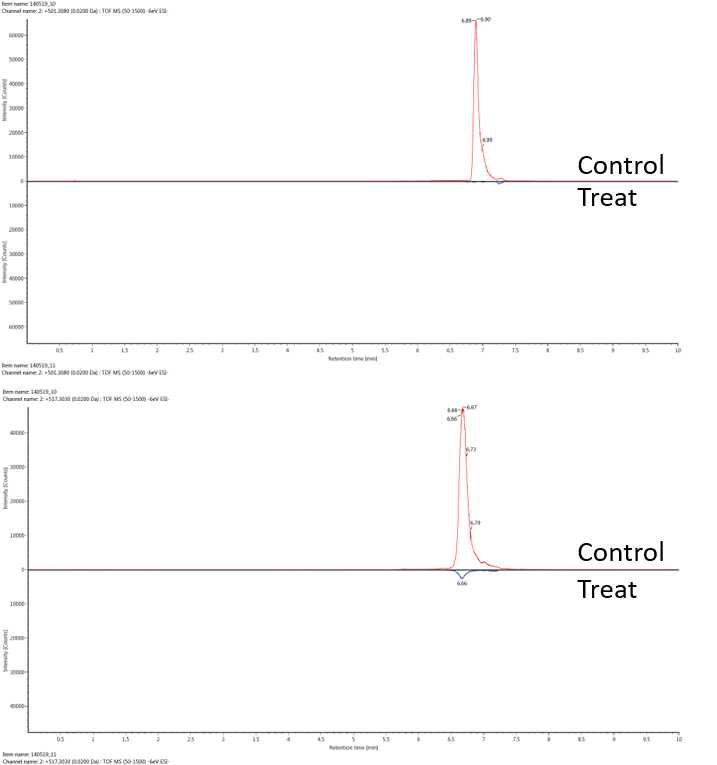
\includegraphics[width=0.7\linewidth]{picture/glucuronate_1}
	\caption{Chromatograms of glucuronates (control and treat) }
	\label{fig:glucuronate1}
\end{figure}
